\section{Architecture}
\label{chap:impl:architecture}


\begin{figure}[tp]
    \centering
    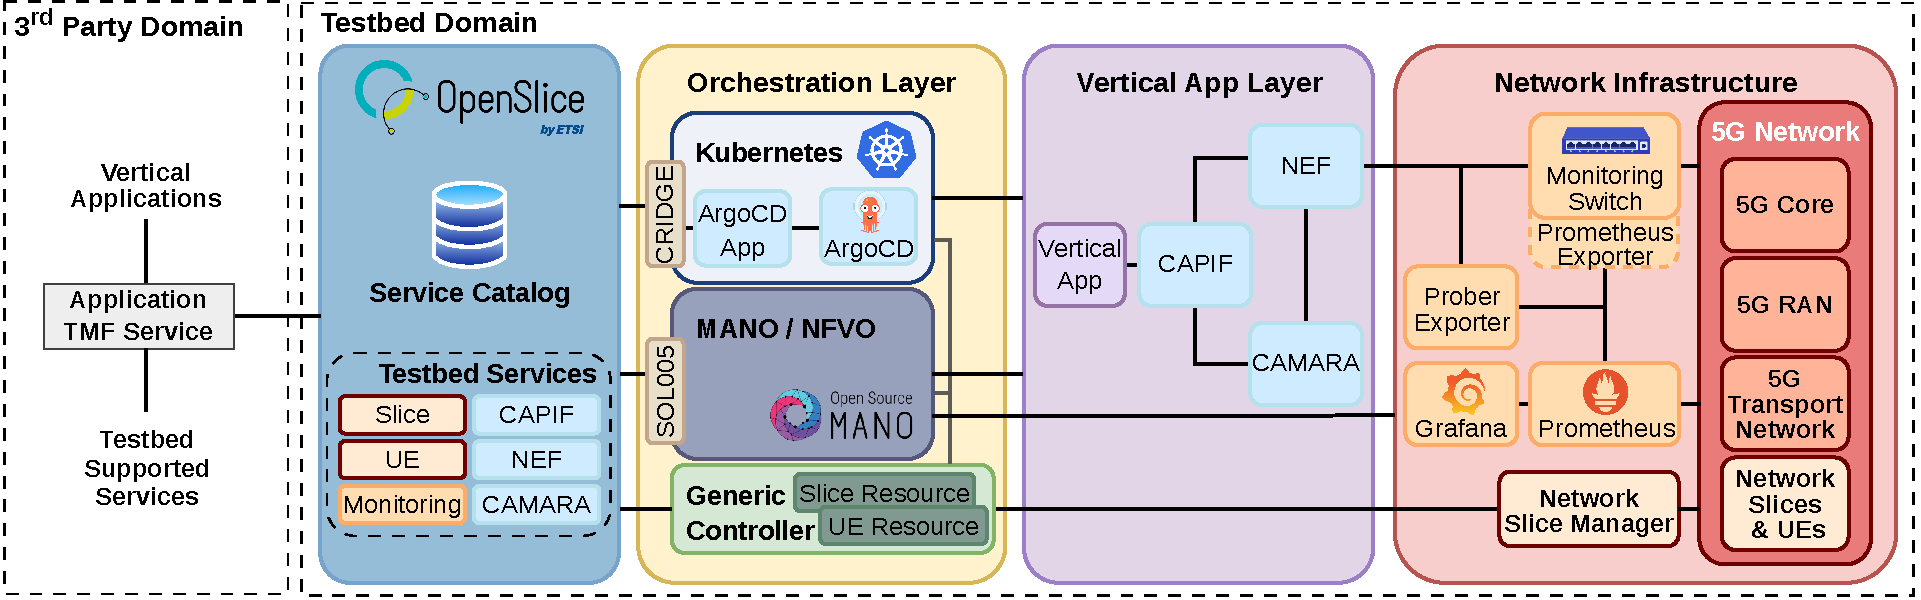
\includegraphics[width=1\linewidth]{figs/drawio/realized_architecture.pdf}
    \caption{Realized Testbed Architecture}
    \label{fig:impl:architecture}
\end{figure}

The proposed testbed is realized on the 5GAIner infrastructure~\cite{5GAIner} at \acs{ITAv}, which provides a commercial-grade standalone \acs{5G} network delivered through multiple \acs{5G} new radio cells and a Huawei \acs{5G} Core compliant with \acs{3GPP} Release 17. The testbed, illustrated in Figure~\ref{fig:impl:architecture}, implements the open, programmable environment proposed in Chapter~\ref{chap:proposal}, providing standardized interfaces to expose the network services offered by the infrastructure. It incorporates the \acs{5G} resource lifecycle management, network exposure, monitoring, and service provisioning capabilities highlighted in the proposal, identifying the concrete components that deliver each of the proposed functionalities. Combined, these components support the development and validation of applications by vertical industries and, consequently, of the exposure interfaces and underlying capabilities provided by the testbed.

Within the network exposure layer, the \acs{NEF}, proposed in Section~\ref{chap:proposal:architecture} as the main gateway for \acs{5G} programmability, establishes the foundation for the remaining exposure components. Due to the wide variety of \acs{5GC} implementations, an analysis of the various \acs{NEF} implementations was conducted in Section \ref{exposure:NEFimplementations}. Based on this analysis, the NEFSim~\cite{NEFSimMediaNetLabGithub}, as extended by \acs{ITAv}~\cite{NEFemulatorAtnog}, was selected as the most suitable choice for the \acs{NEF} implementation, due to its suite of supported northbound \acsp{API} and its integration capabilities with \acs{CAPIF} implementations, compared to its alternatives, as detailed in Section~\ref{chap:impl:exposure:nef}.

In order to further simplify the access to the complex set of network services offered by the NEFSim, CAMARA \acsp{API} are adopted, providing an abstraction layer that facilitates the integration of network capabilities into applications. This way, the CAMARA initative supports the development of network applications that explore the wide variety of use cases enabled through its set of user-friendly \acsp{API}, as described in Section \ref{sec:iniatives:CAMARA}.

Hence, the CAMARA and NEFSim components handle the exposure of network capabilities to third parties. However, there is still a lack of a standardized mechanism for the secure discovery, exposure, and consumption of these northbound \acsp{API}, which is achieved through the introduction of \acs{CAPIF}. More specifically, OpenCAPIF~\cite{OpenCAPIF}, an open source project by the \acs{ETSI} \acs{SDG}, was selected for the implementation of the \acs{CAPIF} framework, as detailed in Section~\ref{chap:impl:exposure:capif}. Thus, OpenCAPIF is utilized to securely expose CAMARA \acsp{API}, as well as \acs{NEF} \acsp{API}, to allow access to all \acs{NEF} functionalities not supported by the CAMARA use cases or that have previously been used for implementation within \acs{ITAv}.

The combination of OpenCAPIF, \acs{NEF} and CAMARA provides standardized secure access to network capabilities across a wide range of use cases. To support this variety of use cases, network slicing is applied to tailor to its heterogeneous service requirements on a common underlying infrastructure. To this end, \acf{OSL}~\cite{OpenSlice} is chosen as the predilect \acs{OSS} to deliver \acs{NaaS}, based on \acs{TMF} \acs{ODA}, since it is widely used in the literature for the provisioning and orchestration of \acs{5G} resources (especially \acsp{UE} and network slices) packaged as \acs{OSL} services, important for testing and validation purposes as showcased in Section \ref{sec:pipelines}. Service orders made to \acs{OSL} are fulfilled by the orchestration layer, being delegated to the \acs{NFVO} \acs{OSM}, for \acs{NFV}-based deployment through the SOL005 interface, or to kubernetes, for containerized deployment through the CRIDGE component. Services packaged as Helm charts, such as the vertical applications, are deployed on kubernetes through Argo CD. The \acs{NSMF} and \acs{NSSMF} roles defined in the proprosal are abstracted by the proprietary \acs{ITAv} Slice Manager, which provisions network slices and \acsp{UE} on the \acs{5G} system. \acs{OSL}, inspired by the Operator Pattern, also supports Generic Controllers to automate the lifecycle management of custom resources~\cite{OpenSliceGenericServicesController}. These are leveraged to implement the lifecycle logic for the \acs{NSI} as discussed in Section \ref{sec:slice:lifecycle}, as well as that of the \acsp{UE}. Such Generic Controllers are responsible for the creation, update and deletion of the aforementioned resources in the 5GAIner testbed by interacting with the Slice Manager, which in turn interacts with the \acs{5G} System (\acs{5GC} and \acs{RAN}), as detailed in Section~\ref{chap:impl:resource_lifecycle}.

It is also important to note the existence of a telemetry monitoring stack utilizing Prometheus exporters and Grafana for the collection and visualization of network metrics, respectively, as defined in Section~\ref{chap:proposal:observability}. Passive monitoring relies on a Prometheus exporter collecting traffic metrics from the \acs{5G} network, while active monitoring relies on a prober exporter measuring \acs{RTT}, packet loss and \acs{RTT} jitter. The collected metrics are stored in Prometheus, acting as the testbed's \acs{TSDB} for storing and querying network analytics. 

The result is an open, programmable environment in which vertical industries can develop and validate applications that interact with the \acs{5G} system.
